\begin{comment}
\chapter{Dynamic programming}

\index{dynamic programming}

\key{Dynamic programming}
is a technique that combines the correctness
of complete search and the efficiency
of greedy algorithms.
Dynamic programming can be applied if the
problem can be divided into overlapping subproblems
that can be solved independently.

There are two uses for dynamic programming:

\begin{itemize}
\item
\key{Finding an optimal solution}:
We want to find a solution that is
as large as possible or as small as possible.
\item
\key{Counting the number of solutions}:
We want to calculate the total number of
possible solutions.
\end{itemize}
\end{comment}


\chapter{動的計画法}

\index{dynamic programming}
\index{動的計画法}

動的計画法(\key{Dynamic programming})は、全探索の正確さと
貪欲アルゴリズムの効率を組み合わせたテクニックである。
動的計画法が適用できるのは、元の問題を個々に解くことができる部分問題に
分割できる場合である。

動的計画法には2つの用途がある:

\begin{itemize}
\item
\key{最適解の発見}:
できるだけ大きい解、もしくはできるだけ小さい解を見つけたい。
\item
\key{解の数え上げ}:
条件を満たす解の総数を計算したい。
\end{itemize}

\begin{comment}
We will first see how dynamic programming can
be used to find an optimal solution,
and then we will use the same idea for
counting the solutions.

Understanding dynamic programming is a milestone
in every competitive programmer's career.
While the basic idea is simple,
the challenge is how to apply
dynamic programming to different problems.
This chapter introduces a set of classic problems
that are a good starting point.
\end{comment}

まず、動的計画法が最適解を探す例と、数え上げを行う例を見ていこう。

動的計画法の理解は、すべての競技プログラミング参加者の
マイルストーンである。
動的計画法の基本的アイデアは非常にシンプルだが、
個々の問題にどのように適用するかという点にむずかしさがある。
本章では、スタート地点として良い題材となる古典的問題を紹介していこう。

\begin{comment}
\section{Coin problem}

We first focus on a problem that we
have already seen in Chapter 6:
Given a set of coin values $\texttt{coins} = \{c_1,c_2,\ldots,c_k\}$
and a target sum of money $n$, our task is to
form the sum $n$ using as few coins as possible.

In Chapter 6, we solved the problem using a
greedy algorithm that always chooses the largest
possible coin.
The greedy algorithm works, for example,
when the coins are the euro coins,
but in the general case the greedy algorithm
does not necessarily produce an optimal solution.
\end{comment}

\section{コイン問題}

ここではすでに6章で見た問題を再度題材とする。
価値が$\texttt{coins} = \{c_1,c_2,\ldots,c_k\}$であるコインが与えられ、
目的の金額$n$が与えられたとき、総額が$n$となる
最小枚数のコインを求める問題である。

6章では、我々はこの問題を常に選びうる最大金額の
コインを選ぶという貪欲アルゴリズムで解いた。
あの貪欲アルゴリズムは、例えばユーロと同じ金額の配分であれば
うまくいくが、一般的にあのアルゴリズムは最適解を必ず
生成するとは限らない。

\begin{comment}
Now is time to solve the problem efficiently
using dynamic programming, so that the algorithm
works for any coin set.
The dynamic programming
algorithm is based on a recursive function
that goes through all possibilities how to
form the sum, like a brute force algorithm.
However, the dynamic programming
algorithm is efficient because
it uses \emph{memoization} and
calculates the answer to each subproblem only once.
\end{comment}

ここでは、あらゆるコイン群に対しうまく動作する、
動的計画法を使った効率的な解法を考えよう。
動的計画法のアルゴリズムは、総当たりのように
全ての組み合わせを探索する再帰関数に基づく。
しかし動的計画法のアルゴリズムでは、\emph{メモ化}により
同じ部分問題を繰り返し計算することを避けることにより
効率化する。

\begin{comment}
\subsubsection{Recursive formulation}

The idea in dynamic programming is to
formulate the problem recursively so
that the solution to the problem can be
calculated from solutions to smaller
subproblems.
In the coin problem, a natural recursive
problem is as follows:
what is the smallest number of coins
required to form a sum $x$?
\end{comment}

\subsubsection{漸化式の作成}

動的計画法のアイデアは、問題を再帰的に定式化し、
より小さな問題の解を用いて元の問題の解を得ることである。
コインの問題では、最初の問題はこのようになる:
合計金額を$x$とする必要なコインの最小枚数は?

\begin{comment}
Let $\texttt{solve}(x)$
denote the minimum
number of coins required for a sum $x$.
The values of the function depend on the
values of the coins.
For example, if $\texttt{coins} = \{1,3,4\}$,
the first values of the function are as follows:
\end{comment}

$\texttt{solve}(x)$を合計金額$x$を満たすのに必要な
コインの最小枚数とする。
この関数の値は、個々のコインの額による。
例えば、コインの額が$\texttt{coins} = \{1,3,4\}$である場合、
この関数の値は以下の通りとなる:

\[
\begin{array}{lcl}
\texttt{solve}(0) & = & 0 \\
\texttt{solve}(1) & = & 1 \\
\texttt{solve}(2) & = & 2 \\
\texttt{solve}(3) & = & 1 \\
\texttt{solve}(4) & = & 1 \\
\texttt{solve}(5) & = & 2 \\
\texttt{solve}(6) & = & 2 \\
\texttt{solve}(7) & = & 2 \\
\texttt{solve}(8) & = & 2 \\
\texttt{solve}(9) & = & 3 \\
\texttt{solve}(10) & = & 3 \\
\end{array}
\]

\begin{comment}
For example, $\texttt{solve}(10)=3$,
because at least 3 coins are needed
to form the sum 10.
The optimal solution is $3+3+4=10$.

The essential property of $\texttt{solve}$ is
that its values can be
recursively calculated from its smaller values.
The idea is to focus on the \emph{first}
coin that we choose for the sum.
For example, in the above scenario,
the first coin can be either 1, 3 or 4.
If we first choose coin 1,
the remaining task is to form the sum 9
using the minimum number of coins,
which is a subproblem of the original problem.
Of course, the same applies to coins 3 and 4.
Thus, we can use the following recursive formula
to calculate the minimum number of coins:
\end{comment}

例えば$\texttt{solve}(10)=3$である。
なぜなら、合計金額を10とするには3枚のコインがあればよく、
最適解で$3+3+4=10$が存在するためである。

$\texttt{solve}$の重要な性質は、この値はより小さな値から
再帰的に計算できる点である。
ここで合計を計算するにあたり\emph{最初に}選ぶコインに着目してみる。
例えば、先ほどの例では最初に選ぶコインは1, 3, 4のいずれかである。
もし最初に1を選ぶと、残りの問題は合計9を達成する
最小コイン枚数を選ぶ問題となる。
これは元の問題の部分問題となる。
もちろん、同様の議論は3,4のコインにも成り立つ。
よって、最小コイン枚数に関する以下の漸化式が利用できる。
\begin{equation*}
\begin{split}
\texttt{solve}(x) = \min( & \texttt{solve}(x-1)+1, \\
                           & \texttt{solve}(x-3)+1, \\
                           & \texttt{solve}(x-4)+1).
\end{split}
\end{equation*}

\begin{comment}
The base case of the recursion is $\texttt{solve}(0)=0$,
because no coins are needed to form an empty sum.
For example,
\[ \texttt{solve}(10) = \texttt{solve}(7)+1 = \texttt{solve}(4)+2 = \texttt{solve}(0)+3 = 3.\]

Now we are ready to give a general recursive function
that calculates the minimum number of
coins needed to form a sum $x$:
\end{comment}

この漸化式の始まりは$\texttt{solve}(0)=0$である。
合計金額0を満たすのは明らかにコイン0枚であるためである。
よって、例えば以下のように計算できる。
\[ \texttt{solve}(10) = \texttt{solve}(7)+1 = \texttt{solve}(4)+2 = \texttt{solve}(0)+3 = 3.\]

ここから、一般的なコインの組み合わせに関して、
同様に合計金額$x$を満たす最小コイン枚数を求める漸化式が構成できる:
\begin{equation*}
    \texttt{solve}(x) = \begin{cases}
               \infty               & x < 0\\
               0               & x = 0\\
               \min_{c \in \texttt{coins}} \texttt{solve}(x-c)+1 & x > 0 \\
           \end{cases}
\end{equation*}

\begin{comment}
First, if $x<0$, the value is $\infty$,
because it is impossible to form a negative
sum of money.
Then, if $x=0$, the value is $0$,
because no coins are needed to form an empty sum.
Finally, if $x>0$, the variable $c$ goes through
all possibilities how to choose the first coin
of the sum.

Once a recursive function that solves the problem
has been found,
we can directly implement a solution in C++
(the constant \texttt{INF} denotes infinity):
\end{comment}

まず$x<0$の場合、値は$\infty$である。
なぜなら合計金額が負となる選び方は不可能であるためである。
$x=0$の場合、値は$0$となる。
これは合計金額が0となるのにコインは1枚も不要なためである。
最後に$x>0$のとき、変数$c$は1枚目のコインとして選べる
全てのコインに関し探索する。

一度問題を解くための漸化式が構築できれば、
それをC++で直接実装できる
(定数\texttt{INF}は無限大を意味するものとする):

\begin{lstlisting}
int solve(int x) {
    if (x < 0) return INF;
    if (x == 0) return 0;
    int best = INF;
    for (auto c : coins) {
        best = min(best, solve(x-c)+1);
    }
    return best;
}
\end{lstlisting}

\begin{comment}
Still, this function is not efficient,
because there may be an exponential number of ways
to construct the sum.
However, next we will see how to make the
function efficient using a technique called memoization.
\end{comment}

またこの関数は効率的でない。
この式では、解を得るたびに必要な計算回数が指数関数的に増加する
場合があるためである。
次に、メモ化と呼ぶ手法を使いこの関数を効率的にする方法を見ていこう。

\begin{comment}
\subsubsection{Using memoization}

\index{memoization}

The idea of dynamic programming is to use
\key{memoization} to efficiently calculate
values of a recursive function.
This means that the values of the function
are stored in an array after calculating them.
For each parameter, the value of the function
is calculated recursively only once, and after this,
the value can be directly retrieved from the array.

In this problem, we use arrays
\begin{lstlisting}
bool ready[N];
int value[N];
\end{lstlisting}
\end{comment}

\subsubsection{メモ化の利用}

\index{memoization}
\index{メモ化}

動的計画法では、再帰的な関数を効率的に計算するため
メモ化(\key{memoization})を用いる。
これは、関数の値を計算後配列に覚えておき、
同じ入力に対して再度同じ関数が呼び出されたら
その値を取り出して再計算を避ける手法である。

この問題では、以下の配列を使うものとする:
\begin{lstlisting}
bool ready[N];
int value[N];
\end{lstlisting}

\begin{comment}
where $\texttt{ready}[x]$ indicates
whether the value of $\texttt{solve}(x)$ has been calculated,
and if it is, $\texttt{value}[x]$
contains this value.
The constant $N$ has been chosen so
that all required values fit in the arrays.

Now the function can be efficiently
implemented as follows:
\end{comment}

$\texttt{ready}[x]$は$\texttt{solve}(x)$の値が計算済みかどうかを示す。
そして計算済みであれば、$\texttt{value}[x]$にその値を格納する。
定数$N$は必要な値がすべて配列に格納しきれるように選ぶ。

こうすると、先の関数は以下の通り効率的に実装できる:

\begin{lstlisting}
int solve(int x) {
    if (x < 0) return INF;
    if (x == 0) return 0;
    if (ready[x]) return value[x];
    int best = INF;
    for (auto c : coins) {
        best = min(best, solve(x-c)+1);
    }
    value[x] = best;
    ready[x] = true;
    return best;
}
\end{lstlisting}

\begin{comment}
The function handles the base cases
$x<0$ and $x=0$ as previously.
Then the function checks from
$\texttt{ready}[x]$ if
$\texttt{solve}(x)$ has already been stored
in $\texttt{value}[x]$,
and if it is, the function directly returns it.
Otherwise the function calculates the value
of $\texttt{solve}(x)$
recursively and stores it in $\texttt{value}[x]$.

This function works efficiently,
because the answer for each parameter $x$
is calculated recursively only once.
After a value of $\texttt{solve}(x)$ has been stored in $\texttt{value}[x]$,
it can be efficiently retrieved whenever the
function will be called again with the parameter $x$.
The time complexity of the algorithm is $O(nk)$,
where $n$ is the target sum and $k$ is the number of coins.
\end{comment}

この関数では、$x<0$と$x=0$の場合は以前の解法と同じである。
そうでない場合、関数では$\texttt{ready}[x]$をチェックして
$\texttt{solve}(x)$の解がすでに$\texttt{value}[x]$に格納済みか判定する。
格納済みであればその値を返して関数は終了し、
そうでなければ関数は$\texttt{solve}(x)$の値を計算し、
$\texttt{value}[x]$に格納しておく。

この関数は、各入力$x$に対し一度ずつしか再帰的な計算を
行わないため、効率的に動作する。
$\texttt{solve}(x)$の値が$\texttt{value}[x]$に格納された後は、
同じ入力$x$に対しそれを取り出すだけで済むためである。
このアルゴリズムは、合計金額を$n$、コインの種類を$k$とすると
時間計算量$O(nk)$となる。

\begin{comment}
Note that we can also 
construct the array \texttt{value} using
a loop that simply calculates all the values
of $\texttt{solve}$ for parameters $0 \ldots n$:
\end{comment}

なお、入力$0 \ldots n$に対する$\texttt{solve}$の値を、
再帰を使わず単純なループで\emph{繰り返し}構築していくこともできる:

\begin{lstlisting}
value[0] = 0;
for (int x = 1; x <= n; x++) {
    value[x] = INF;
    for (auto c : coins) {
        if (x-c >= 0) {
            value[x] = min(value[x], value[x-c]+1);
        }
    }
}
\end{lstlisting}

\begin{comment}
In fact, most competitive programmers prefer this
implementation, because it is shorter and has
lower constant factors.
From now on, we also use iterative implementations
in our examples.
Still, it is often easier to think about
dynamic programming solutions
in terms of recursive functions.
\end{comment}

実際、多くの競技プログラマはこちらの実装の方が短く
定数倍高速なためこちらの書き方を好む。
以降、本書で例を示す際、こちらのループによる実装も使用していく。
しかし、動的計画法は再帰的な関数の観点で解を考えた方が
易しい場合もある。

\begin{comment}
\subsubsection{Constructing a solution}

Sometimes we are asked both to find the value
of an optimal solution and to give
an example how such a solution can be constructed.
In the coin problem, for example,
we can declare another array
that indicates for
each sum of money the first coin 
in an optimal solution:
\begin{lstlisting}
int first[N];
\end{lstlisting}
Then, we can modify the algorithm as follows:
\end{comment}

\subsubsection{解の構築}

時々、最適値を求めるだけでなく最適値の構成例を
求める問題に出会うことがある。
コインの問題では、例えば別の配列に求める総額を達成するために
最初の1枚で選ぶコインを代入しておくことでこのような問題に
対応することができる:
\begin{lstlisting}
int first[N];
\end{lstlisting}

この配列を使い、先ほどのアルゴリズムをこのように書き換える:
\begin{lstlisting}
value[0] = 0;
for (int x = 1; x <= n; x++) {
    value[x] = INF;
    for (auto c : coins) {
        if (x-c >= 0 && value[x-c]+1 < value[x]) {
            value[x] = value[x-c]+1;
            first[x] = c;
        }
    }
}
\end{lstlisting}

\begin{comment}
After this, the following code can be used to
print the coins that appear in an optimal solution for
the sum $n$:
\end{comment}

その後、以下のコードは合計金額を$n$にするような
コインの構成を出力する:
\begin{lstlisting}
while (n > 0) {
    cout << first[n] << "\n";
    n -= first[n];
}
\end{lstlisting}

\begin{comment}
\subsubsection{Counting the number of solutions}

Let us now consider another version
of the coin problem where our task is to
calculate the total number of ways
to produce a sum $x$ using the coins.
For example, if $\texttt{coins}=\{1,3,4\}$ and
$x=5$, there are a total of 6 ways:
\end{comment}

\subsubsection{解の数え上げ}

今度はコインの問題の別バージョンとして、
合計金額$x$とするコインの選び方が
何通りあるか数える問題を考えよう。

例えば$\texttt{coins}=\{1,3,4\}$ かつ
$x=5$であれば、計6通りの選び方がある;

\begin{multicols}{2}
\begin{itemize}
\item $1+1+1+1+1$
\item $1+1+3$
\item $1+3+1$
\item $3+1+1$
\item $1+4$
\item $4+1$
\end{itemize}
\end{multicols}

\begin{comment}
Again, we can solve the problem recursively.
Let $\texttt{solve}(x)$ denote the number of ways
we can form the sum $x$.
For example, if $\texttt{coins}=\{1,3,4\}$,
then $\texttt{solve}(5)=6$ and the recursive formula is
\end{comment}

こちらも、再帰的に解くことができる。
$\texttt{solve}(x)$ を合計金額を$x$とするコインの選び方の
数とする。
例えば$\texttt{coins}=\{1,3,4\}$であれば$\texttt{solve}(5)=6$である。
この関数に関して、以下のように再帰的に値を計算できる:
\begin{equation*}
\begin{split}
\texttt{solve}(x) = & \texttt{solve}(x-1) + \\
                    & \texttt{solve}(x-3) + \\
                    & \texttt{solve}(x-4)  .
\end{split}
\end{equation*}

\begin{comment}
Then, the general recursive function is as follows:
\end{comment}

コインの種類に関し、一般形はこのように表せる:

\begin{equation*}
    \texttt{solve}(x) = \begin{cases}
               0               & x < 0\\
               1               & x = 0\\
               \sum_{c \in \texttt{coins}} \texttt{solve}(x-c) & x > 0 \\
           \end{cases}
\end{equation*}

\begin{comment}
If $x<0$, the value is 0, because there are no solutions.
If $x=0$, the value is 1, because there is only one way
to form an empty sum.
Otherwise we calculate the sum of all values
of the form $\texttt{solve}(x-c)$ where $c$ is in \texttt{coins}.

The following code constructs an array
$\texttt{count}$ such that
$\texttt{count}[x]$ equals
the value of $\texttt{solve}(x)$
for $0 \le x \le n$:
\end{comment}

もし$x<0$ならば、明らかにそのような構成は存在しないので値は0となる。
$x=0$であれば、コインを何も選ばないという組み合わせのみ存在するので値は1となる。
それ以外の場合、\texttt{coins}に含まれる全ての$c$に対し、
$\texttt{solve}(x-c)$の値を合計したものが値となる。

$\texttt{count}[x]$を$\texttt{solve}(x)$の値を$0 \le x \le n$の範囲で格納する
配列だとすると、この配列はこのように作ることができる:


\begin{lstlisting}
count[0] = 1;
for (int x = 1; x <= n; x++) {
    for (auto c : coins) {
        if (x-c >= 0) {
            count[x] += count[x-c];
        }
    }
}
\end{lstlisting}

\begin{comment}
Often the number of solutions is so large
that it is not required to calculate the exact number
but it is enough to give the answer modulo $m$
where, for example, $m=10^9+7$.
This can be done by changing the code so that
all calculations are done modulo $m$.
In the above code, it suffices to add the line
\begin{lstlisting}
        count[x] %= m;
\end{lstlisting}
after the line
\begin{lstlisting}
        count[x] += count[x-c];
\end{lstlisting}

Now we have discussed all basic
ideas of dynamic programming.
Since dynamic programming can be used
in many different situations,
we will now go through a set of problems
that show further examples about the
possibilities of dynamic programming.
\end{comment}

しばしば求める組わせの数が非常に大きくなるため、
正確な値ではなく代わりにある$m$の剰余、
例えば$m=10^9+7$の剰余を答えさせる問題がある。
この場合、先ほどのコードにおいてすべての計算に$m$の剰余を
求める式を加えるとよい。
先ほどのコードであれば、下記のコードを:
\begin{lstlisting}
        count[x] %= m;
\end{lstlisting}
以下の行の後に加える:
\begin{lstlisting}
        count[x] += count[x-c];
\end{lstlisting}

ここまでで動的計画法の基本アイデアについて述べた。
動的計画法は様々な状況において利用できるため、
その可能性に触れられるいくつかの問題について触れていくことにする。

\begin{comment}
\section{Longest increasing subsequence}

\index{longest increasing subsequence}

Our first problem is to find the
\key{longest increasing subsequence}
in an array of $n$ elements.
This is a maximum-length
sequence of array elements
that goes from left to right,
and each element in the sequence is larger
than the previous element.
For example, in the array
\end{comment}

\section{最長増加部分列}

\index{longest increasing subsequence}
\index{最長増加部分列}

最初の問題は、$n$要素の配列における
最長増加部分列(\key{longest increasing subsequence})を見つける問題である。
最長増加部分列とは、元の数列の部分列のうち、選んだ要素を
順に並べると手前の要素より後の要素の方が大きいという条件を満たす
最長のものである。

例えば、以下の数列において:
\begin{center}
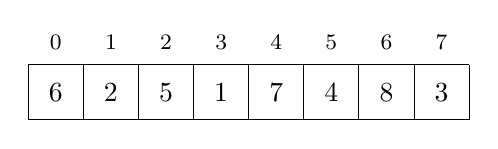
\begin{tikzpicture}[scale=0.7]
\draw (0,0) grid (8,1);
\node at (0.5,0.5) {$6$};
\node at (1.5,0.5) {$2$};
\node at (2.5,0.5) {$5$};
\node at (3.5,0.5) {$1$};
\node at (4.5,0.5) {$7$};
\node at (5.5,0.5) {$4$};
\node at (6.5,0.5) {$8$};
\node at (7.5,0.5) {$3$};

\footnotesize
\node at (0.5,1.4) {$0$};
\node at (1.5,1.4) {$1$};
\node at (2.5,1.4) {$2$};
\node at (3.5,1.4) {$3$};
\node at (4.5,1.4) {$4$};
\node at (5.5,1.4) {$5$};
\node at (6.5,1.4) {$6$};
\node at (7.5,1.4) {$7$};
\end{tikzpicture}
\end{center}

\begin{comment}
the longest increasing subsequence
contains 4 elements:
\end{comment}

最長増加部分列は4要素からなる:
\begin{center}
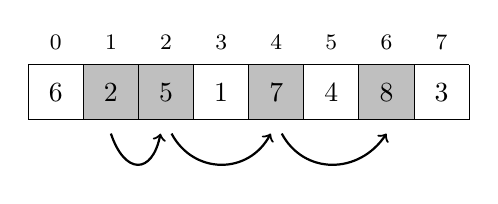
\begin{tikzpicture}[scale=0.7]
\fill[color=lightgray] (1,0) rectangle (2,1);
\fill[color=lightgray] (2,0) rectangle (3,1);
\fill[color=lightgray] (4,0) rectangle (5,1);
\fill[color=lightgray] (6,0) rectangle (7,1);
\draw (0,0) grid (8,1);
\node at (0.5,0.5) {$6$};
\node at (1.5,0.5) {$2$};
\node at (2.5,0.5) {$5$};
\node at (3.5,0.5) {$1$};
\node at (4.5,0.5) {$7$};
\node at (5.5,0.5) {$4$};
\node at (6.5,0.5) {$8$};
\node at (7.5,0.5) {$3$};

\draw[thick,->] (1.5,-0.25) .. controls (1.75,-1.00) and (2.25,-1.00) .. (2.4,-0.25);
\draw[thick,->] (2.6,-0.25) .. controls (3.0,-1.00) and (4.0,-1.00) .. (4.4,-0.25);
\draw[thick,->] (4.6,-0.25) .. controls (5.0,-1.00) and (6.0,-1.00) .. (6.5,-0.25);

\footnotesize
\node at (0.5,1.4) {$0$};
\node at (1.5,1.4) {$1$};
\node at (2.5,1.4) {$2$};
\node at (3.5,1.4) {$3$};
\node at (4.5,1.4) {$4$};
\node at (5.5,1.4) {$5$};
\node at (6.5,1.4) {$6$};
\node at (7.5,1.4) {$7$};
\end{tikzpicture}
\end{center}

\begin{comment}
Let $\texttt{length}(k)$ denote
the length of the
longest increasing subsequence
that ends at position $k$.
Thus, if we calculate all values of
$\texttt{length}(k)$ where $0 \le k \le n-1$,
we will find out the length of the
longest increasing subsequence.
For example, the values of the function
for the above array are as follows:
\end{comment}


$\texttt{length}(k)$を、$k$番目の要素を終端とする
最長増加部分列の長さとする。
$\texttt{length}(k)$の値を$0 \le k \le n-1$全てについて
求めていくことにする。
先ほどの例では、この関数の値は以下のようになる:
\[
\begin{array}{lcl}
\texttt{length}(0) & = & 1 \\
\texttt{length}(1) & = & 1 \\
\texttt{length}(2) & = & 2 \\
\texttt{length}(3) & = & 1 \\
\texttt{length}(4) & = & 3 \\
\texttt{length}(5) & = & 2 \\
\texttt{length}(6) & = & 4 \\
\texttt{length}(7) & = & 2 \\
\end{array}
\]

\begin{comment}
For example, $\texttt{length}(6)=4$,
because the longest increasing subsequence
that ends at position 6 consists of 4 elements.

To calculate a value of $\texttt{length}(k)$,
we should find a position $i<k$
for which $\texttt{array}[i]<\texttt{array}[k]$
and $\texttt{length}(i)$ is as large as possible.
Then we know that
$\texttt{length}(k)=\texttt{length}(i)+1$,
because this is an optimal way to add
$\texttt{array}[k]$ to a subsequence.
However, if there is no such position $i$,
then $\texttt{length}(k)=1$,
which means that the subsequence only contains
$\texttt{array}[k]$.
\end{comment}

例えば$\texttt{length}(6)=4$となるのは、
6番目の要素を終端とする最長増加部分列は
4要素で構成されることを意味する。

$\texttt{length}(k)$を求めるためには、
$i<k$かつ$\texttt{array}[i]<\texttt{array}[k]$となる$i$のうち、
$\texttt{length}(i)$が最大のものを見つけられれば良い。
そうすれば、$i$番目の要素を末尾とする最長部分増加列に
$k$番目の値を追加することで、$\texttt{length}(k)=\texttt{length}(i)+1$が
得られることがわかる。
そのようなiが1つも存在しない場合、$\texttt{length}(k)=1$、すなわち
$k$番目の要素だけで構成される部分列しか構成できない。

\begin{comment}
Since all values of the function can be calculated
from its smaller values,
we can use dynamic programming.
In the following code, the values
of the function will be stored in an array
$\texttt{length}$.
\end{comment}

この関数の値は、より小さな引数の結果から計算できるため、
動的計画法が適用できる。
以下のコードでは、先ほどの関数の値は配列
$\texttt{length}$に格納される。

\begin{lstlisting}
for (int k = 0; k < n; k++) {
    length[k] = 1;
    for (int i = 0; i < k; i++) {
        if (array[i] < array[k]) {
            length[k] = max(length[k],length[i]+1);
        }
    }
}
\end{lstlisting}

\begin{comment}
This code works in $O(n^2)$ time,
because it consists of two nested loops.
However, it is also possible to implement
the dynamic programming calculation
more efficiently in $O(n \log n)$ time.
Can you find a way to do this?
\end{comment}

このコードは二重ループであり時間計算量$O(n^2)$で動く。
しかしこの処理はより効率的に時間計算量$O(n \log n)$で
処理できるアルゴリズムが存在する。
あなたはそのような方法がわかるだろうか?

\begin{comment}
\section{Paths in a grid}

Our next problem is to find a path
from the upper-left corner to
the lower-right corner
of an $n \times n$ grid, such that
we only move down and right.
Each square contains a positive integer,
and the path should be constructed so
that the sum of the values along
the path is as large as possible.
\end{comment}

\section{グリッド中のパス}

次の問題は、$n \times n$のグリッドにおいて、
左上角のマスから始めて、右または下に移動しながら
右下角のマスに到達するパスを見つける問題である。
各マスには正整数が書かれており、
経由したマスに書かれた整数の総和が最大となる
パスを求めることを考えよう。

\begin{comment}
The following picture shows an optimal
path in a grid:
\end{comment}

以下の絵はあるグリッドにおける最適手を示す:
\begin{center}
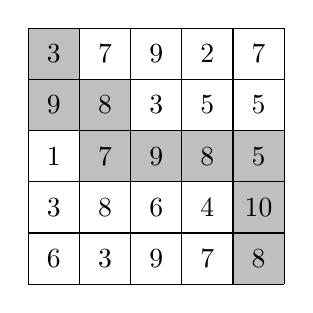
\begin{tikzpicture}[scale=.65]
  \begin{scope}
    \fill [color=lightgray] (0, 9) rectangle (1, 8);
    \fill [color=lightgray] (0, 8) rectangle (1, 7);
    \fill [color=lightgray] (1, 8) rectangle (2, 7);
    \fill [color=lightgray] (1, 7) rectangle (2, 6);
    \fill [color=lightgray] (2, 7) rectangle (3, 6);
    \fill [color=lightgray] (3, 7) rectangle (4, 6);
    \fill [color=lightgray] (4, 7) rectangle (5, 6);
    \fill [color=lightgray] (4, 6) rectangle (5, 5);
    \fill [color=lightgray] (4, 5) rectangle (5, 4);
    \draw (0, 4) grid (5, 9);
    \node at (0.5,8.5) {3};
    \node at (1.5,8.5) {7};
    \node at (2.5,8.5) {9};
    \node at (3.5,8.5) {2};
    \node at (4.5,8.5) {7};
    \node at (0.5,7.5) {9};
    \node at (1.5,7.5) {8};
    \node at (2.5,7.5) {3};
    \node at (3.5,7.5) {5};
    \node at (4.5,7.5) {5};
    \node at (0.5,6.5) {1};
    \node at (1.5,6.5) {7};
    \node at (2.5,6.5) {9};
    \node at (3.5,6.5) {8};
    \node at (4.5,6.5) {5};
    \node at (0.5,5.5) {3};
    \node at (1.5,5.5) {8};
    \node at (2.5,5.5) {6};
    \node at (3.5,5.5) {4};
    \node at (4.5,5.5) {10};
    \node at (0.5,4.5) {6};
    \node at (1.5,4.5) {3};
    \node at (2.5,4.5) {9};
    \node at (3.5,4.5) {7};
    \node at (4.5,4.5) {8};
  \end{scope}
\end{tikzpicture}
\end{center}

\begin{comment}
The sum of the values on the path is 67,
and this is the largest possible sum on a path
from the
upper-left corner to the lower-right corner.
\end{comment}

この図のパスにおける整数の和は67であり、
これは最大である。

\begin{comment}
Assume that the rows and columns of the
grid are numbered from 1 to $n$,
and $\texttt{value}[y][x]$ equals the value
of square $(y,x)$.
Let $\texttt{sum}(y,x)$ denote the maximum
sum on a path from the upper-left corner
to square $(y,x)$.
Now $\texttt{sum}(n,n)$ tells us
the maximum sum
from the upper-left corner to
the lower-right corner.
For example, in the above grid,
$\texttt{sum}(5,5)=67$.
\end{comment}

グリッドの行と列を1から$n$まで番号を振り、
$\texttt{value}[y][x]$をマス$(y,x)$に書かれた値とする。
$\texttt{sum}(y,x)$を左上マスからマス$(y,x)$に至るパスにおける
経由したマスの整数値の総和の最大値とする。
$\texttt{sum}(n,n)$は元の問題で求めたかった値に相当する。
先ほどの例では$\texttt{sum}(5,5)=67$となる。

\begin{comment}
We can recursively calculate the sums
as follows:
\[ \texttt{sum}(y,x) = \max(\texttt{sum}(y,x-1),\texttt{sum}(y-1,x))+\texttt{value}[y][x]\]


The recursive formula is based on the observation
that a path that ends at square $(y,x)$
can come either from square $(y,x-1)$
or square $(y-1,x)$:
\end{comment}

この値は、このように再帰的に求めることができる:
\[ \texttt{sum}(y,x) = \max(\texttt{sum}(y,x-1),\texttt{sum}(y-1,x))+\texttt{value}[y][x]\]

この漸化式は、マス$(y,x)$を終端とするパスは、
直前$(y,x-1)$か$(y-1,x)$いずれかのマスから
来るという考察により得られる:
\begin{center}
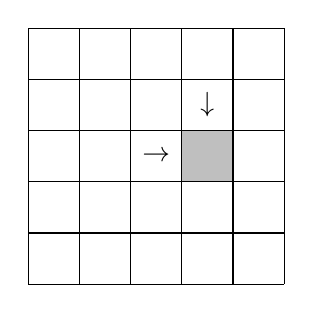
\begin{tikzpicture}[scale=.65]
  \begin{scope}
    \fill [color=lightgray] (3, 7) rectangle (4, 6);
    \draw (0, 4) grid (5, 9);
    
    \node at (2.5,6.5) {$\rightarrow$};
    \node at (3.5,7.5) {$\downarrow$};
    
  \end{scope}
\end{tikzpicture}
\end{center}

\begin{comment}
Thus, we select the direction that maximizes
the sum.
We assume that $\texttt{sum}(y,x)=0$
if $y=0$ or $x=0$ (because no such paths exist),
so the recursive formula also works when $y=1$ or $x=1$.

Since the function \texttt{sum} has two parameters,
the dynamic programming array also has two dimensions.
For example, we can use an array
\begin{lstlisting}
int sum[N][N];
\end{lstlisting}
and calculate the sums as follows:
\begin{lstlisting}
for (int y = 1; y <= n; y++) {
    for (int x = 1; x <= n; x++) {
        sum[y][x] = max(sum[y][x-1],sum[y-1][x])+value[y][x];
    }
}
\end{lstlisting}
The time complexity of the algorithm is $O(n^2)$.
\end{comment}

そのため、和が最大となる方向を選ぶことができる。
$y=0$かつ$x=0$の場合、$\texttt{sum}(y,x)=0$と置くことにすると、
この漸化式は$y=1$や$x=1$の場合にも適用できる。

この関数\texttt{sum}は2つの引数を持ち、
この動的計画法の配列は2次元である。
例えば以下の配列を使うと:
\begin{lstlisting}
int sum[N][N];
\end{lstlisting}

関数の値は以下のように求めることができる:
\begin{lstlisting}
for (int y = 1; y <= n; y++) {
    for (int x = 1; x <= n; x++) {
        sum[y][x] = max(sum[y][x-1],sum[y-1][x])+value[y][x];
    }
}
\end{lstlisting}
このアルゴリズムの時間計算量は$O(n^2)$となる。

\begin{comment}
\section{Knapsack problems}

\index{knapsack}

The term \key{knapsack} refers to problems where
a set of objects is given, and 
subsets with some properties
have to be found.
Knapsack problems can often be solved
using dynamic programming.

In this section, we focus on the following
problem: Given a list of weights
$[w_1,w_2,\ldots,w_n]$,
determine all
sums that can be constructed using the weights.
For example, if the weights are
$[1,3,3,5]$, the following sums are possible:
\end{comment}

\section{ナップサック問題}

\index{knapsack}
\index{ナップサック問題}

ナップサック問題(\key{knapsack})は、
物の集合が与えられて、ある特徴を満たす部分集合を求める
類の問題を指す。
ナップサック問題はしばしば動的計画法で解くことができる。

この節では、以下の問題に着目していく:
$n$個の重りの重さからなる配列$[w_1,w_2,\ldots,w_n]$が与えられる。
この重りの部分集合の総和として得られる重さをすべて列挙せよ。
例えば重さが$[1,3,3,5]$の場合、以下の和を得ることができる。

\begin{center}
\begin{tabular}{rrrrrrrrrrrrr}
 0 & 1 & 2 & 3 & 4 & 5 & 6 & 7 & 8 & 9 & 10 & 11 & 12 \\
\hline
 X & X & & X & X & X & X & X & X & X & & X & X \\
\end{tabular}
\end{center}

\begin{comment}
In this case, all sums between $0 \ldots 12$
are possible, except 2 and 10.
For example, the sum 7 is possible because we
can select the weights $[1,3,3]$.

To solve the problem, we focus on subproblems
where we only use the first $k$ weights
to construct sums.
Let $\texttt{possible}(x,k)=\textrm{true}$ if
we can construct a sum $x$
using the first $k$ weights,
and otherwise $\texttt{possible}(x,k)=\textrm{false}$.
The values of the function can be recursively
calculated as follows:
\[ \texttt{possible}(x,k) = \texttt{possible}(x-w_k,k-1) \lor \texttt{possible}(x,k-1) \]
The formula is based on the fact that we can
either use or not use the weight $w_k$ in the sum.
If we use $w_k$, the remaining task is to
form the sum $x-w_k$ using the first $k-1$ weights,
and if we do not use $w_k$,
the remaining task is to form the sum $x$
using the first $k-1$ weights.
As the base cases,
\end{comment}

この例では、$0 \ldots 12$の範囲では2と10を除いた和が構成可能である。
例えば部分集合として$[1,3,3]$を選べば和として7を得られる。

この問題を解くため、部分問題として最初のk個の重りだけを使って得られる
重さの総和を考えよう。
最初の$k$個の重りの部分集合で重さの和を$x$にできるとき、
$\texttt{possible}(x,k)=\textrm{true}$、そうでないとき
$\texttt{possible}(x,k)=\textrm{false}$とする。
この関数の値は、以下のように再帰的に求めることができる:
\[ \texttt{possible}(x,k) = \texttt{possible}(x-w_k,k-1) \lor \texttt{possible}(x,k-1) \]
この式は、$k$個目の重りの重さ$w_k$を和に含める場合と含めない場合
両方を考えることで導出できる。
もし$w_k$を含めるなら、残りは$x-w_k$の重さを最初の$k-1$個の重りで
構成しなければならないし、$w_k$を含めないなら$x$を最初の$k-1$個の重りで
構成しなければならない。
まず基本的なケースとして以下が成り立つ:
\begin{equation*}
    \texttt{possible}(x,0) = \begin{cases}
               \textrm{true}    & x = 0\\
               \textrm{false}   & x \neq 0 \\
           \end{cases}
\end{equation*}

\begin{comment}
because if no weights are used,
we can only form the sum 0.


The following table shows all values of the function
for the weights $[1,3,3,5]$ :
\end{comment}

これは重りを1つも使わないなら、和は0にしかなりえないためである。

以下の表は、重さの配列が$[1,3,3,5]$であるとき、
対応する関数の値を列挙したものである
(記号 ''X'' はtrueであることを示す):

\begin{center}
\begin{tabular}{r|rrrrrrrrrrrrr}
$k \backslash x$ & 0 & 1 & 2 & 3 & 4 & 5 & 6 & 7 & 8 & 9 & 10 & 11 & 12 \\
\hline
 0 & X & \\
 1 & X & X \\
 2 & X & X & & X & X \\
 3 & X & X & & X & X & & X & X \\
 4 & X & X & & X & X & X & X & X & X & X & & X & X \\
\end{tabular}
\end{center}

\begin{comment}
After calculating those values, $\texttt{possible}(x,n)$
tells us whether we can construct a
sum $x$ using \emph{all} weights.

Let $W$ denote the total sum of the weights.
The following $O(nW)$ time
dynamic programming solution
corresponds to the recursive function:
\end{comment}

これらの値を計算し終えると、$\texttt{possible}(x,n)$が
\emph{全ての}重りを利用した場合、和を$x$にできるかどうかを示すことになる。

全ての重りの重さの総和を$W$とすると、動的計画法により
このテーブルを埋めるための時間計算量は$O(nW)$となる。
対応するコードは以下の通り:
\begin{lstlisting}
possible[0][0] = true;
for (int k = 1; k <= n; k++) {
    for (int x = 0; x <= W; x++) {
        if (x-w[k] >= 0) possible[x][k] |= possible[x-w[k]][k-1];
        possible[x][k] |= possible[x][k-1];
    }
}
\end{lstlisting}

\begin{comment}
However, here is a better implementation that only uses
a one-dimensional array $\texttt{possible}[x]$
that indicates whether we can construct a subset with sum $x$.
The trick is to update the array from right to left for
each new weight:
\end{comment}

ここで、1次元配列$\texttt{possible}[x]$を使ったより
良い実装法もある。
この配列は、和が$x$となる部分集合を構築可能かどうかを示す。
ここで重要なテクニックは、新しい重りに対する処理を、
配列の右から左に更新していくことである:
\begin{lstlisting}
possible[0] = true;
for (int k = 1; k <= n; k++) {
    for (int x = W; x >= 0; x--) {
        if (possible[x]) possible[x+w[k]] = true;
    }
}
\end{lstlisting}

\begin{comment}
Note that the general idea presented here can be used
in many knapsack problems.
For example, if we are given objects with weights and values,
we can determine for each weight sum the maximum value
sum of a subset.
\end{comment}

ここで紹介した基本的なアイデアは、多くのナップサック問題で利用できる。
例えば、商品の重さと価値が与えられたとき、
重さの総和に対し価値を最大化する場合などに適用できる。

\begin{comment}
\section{Edit distance}

\index{edit distance}
\index{Levenshtein distance}

The \key{edit distance} or \key{Levenshtein distance}\footnote{The distance
is named after V. I. Levenshtein who studied it in connection with binary codes \cite{lev66}.}
is the minimum number of editing operations
needed to transform a string
into another string.
The allowed editing operations are as follows:
\begin{itemize}
\item insert a character (e.g. \texttt{ABC} $\rightarrow$ \texttt{ABCA})
\item remove a character (e.g. \texttt{ABC} $\rightarrow$ \texttt{AC})
\item modify a character (e.g. \texttt{ABC} $\rightarrow$ \texttt{ADC})
\end{itemize}

For example, the edit distance between
\texttt{LOVE} and \texttt{MOVIE} is 2,
because we can first perform the operation
 \texttt{LOVE} $\rightarrow$ \texttt{MOVE}
(modify) and then the operation
\texttt{MOVE} $\rightarrow$ \texttt{MOVIE}
(insert).
This is the smallest possible number of operations,
because it is clear that only one operation is not enough.
\end{comment}

\section{編集距離}

\index{edit distance}
\index{Levenshtein distance}
\index{編集距離}
\index{レーベンスタイン距離}

編集距離(\key{edit distance})またはレーベンスタイン距離(\key{Levenshtein distance})
\footnote{この名前は、この問題に取り組んだV. I. Levenshteinに由来する\cite{lev66}.}
は、ある文字列を別の文字列に変換するときに必要な編集回数の最小値である。
1回の編集では、文字列に対し下記のいずれかの処理を行える:
\begin{itemize}
\item 文字を1つ挿入する (例: \texttt{ABC} $\rightarrow$ \texttt{ABCA})
\item 文字を1つ取り除く (例: \texttt{ABC} $\rightarrow$ \texttt{AC})
\item 文字を1つ変更する (例: \texttt{ABC} $\rightarrow$ \texttt{ADC})
\end{itemize}

例えば、\texttt{LOVE}と\texttt{MOVIE}の編集距離は2である。
まず最初の編集で文字の変更により\texttt{LOVE} $\rightarrow$ \texttt{MOVE}となり、
続けて文字の挿入により\texttt{MOVE} $\rightarrow$ \texttt{MOVIE}とできる。
この例では明らかに1回の編集では終えられないので、2が最小値であることがわかる。

\begin{comment}
Suppose that we are given a string \texttt{x}
of length $n$ and a string \texttt{y} of length $m$,
and we want to calculate the edit distance between
\texttt{x} and \texttt{y}.
To solve the problem, we define a function
$\texttt{distance}(a,b)$ that gives the
edit distance between prefixes
$\texttt{x}[0 \ldots a]$ and $\texttt{y}[0 \ldots b]$.
Thus, using this function, the edit distance
between \texttt{x} and \texttt{y} equals $\texttt{distance}(n-1,m-1)$.

We can calculate values of \texttt{distance}
as follows:
\end{comment}

以下、長さ$n$の文字列\texttt{x}と、長さ$m$の文字列\texttt{y}に対し、
\texttt{x}と\texttt{y}の編集距離を求めよう。
問題を解くために、関数$\texttt{distance}(a,b)$を定義する。
この関数は、接頭辞$\texttt{x}[0 \ldots a]$と$\texttt{y}[0 \ldots b]$の
編集距離を返すものとする。
この関数を使えば、求める編集距離$\texttt{distance}(n-1,m-1)$となる。

この関数の値はこのように計算できる:
\begin{equation*}
\begin{split}
\texttt{distance}(a,b) = \min(& \texttt{distance}(a,b-1)+1, \\
                           & \texttt{distance}(a-1,b)+1, \\
                           & \texttt{distance}(a-1,b-1)+\texttt{cost}(a,b)).
\end{split}
\end{equation*}

\begin{comment}
Here $\texttt{cost}(a,b)=0$ if $\texttt{x}[a]=\texttt{y}[b]$,
and otherwise $\texttt{cost}(a,b)=1$.
The formula considers the following ways to
edit the string \texttt{x}:
\begin{itemize}
\item $\texttt{distance}(a,b-1)$: insert a character at the end of \texttt{x}
\item $\texttt{distance}(a-1,b)$: remove the last character from \texttt{x}
\item $\texttt{distance}(a-1,b-1)$: match or modify the last character of \texttt{x}
\end{itemize}
\end{comment}

ここで、$\texttt{x}[a]=\texttt{y}[b]$なら$\texttt{cost}(a,b)=0$、
そうでなければ$\texttt{cost}(a,b)=1$とする。
文字列\texttt{x}に対し1文字加工するケースを考える:
\begin{itemize}
\item $\texttt{distance}(a,b-1)$: \texttt{x}の末尾に文字を加える
\item $\texttt{distance}(a-1,b)$: \texttt{x}の末尾の文字を取り除く
\item $\texttt{distance}(a-1,b-1)$: \texttt{x}の末尾の文字が一致する、または編集する
\end{itemize}

\begin{comment}
In the two first cases, one editing operation is needed
(insert or remove).
In the last case, if $\texttt{x}[a]=\texttt{y}[b]$,
we can match the last characters without editing,
and otherwise one editing operation is needed (modify).

The following table shows the values of \texttt{distance}
in the example case:

\end{comment}

最初の2つのケースでは、1回の編集(挿入または削除)が必要である。
最後のケースでは、$\texttt{x}[a]=\texttt{y}[b]$であれば最後の文字に関しては編集は不要である。
そうでない場合、1回の編集(変更)が必要となる。

以下の表は、上記例における\texttt{distance}の値を示す:
\begin{center}
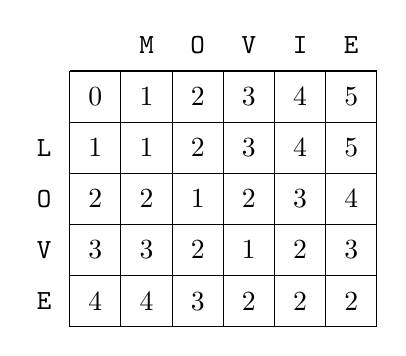
\begin{tikzpicture}[scale=.65]
  \begin{scope}
    %\fill [color=lightgray] (5, -3) rectangle (6, -4);
    \draw (1, -1) grid (7, -6);
    
    \node at (0.5,-2.5) {\texttt{L}};
    \node at (0.5,-3.5) {\texttt{O}};
    \node at (0.5,-4.5) {\texttt{V}};
    \node at (0.5,-5.5) {\texttt{E}};

    \node at (2.5,-0.5) {\texttt{M}};
    \node at (3.5,-0.5) {\texttt{O}};
    \node at (4.5,-0.5) {\texttt{V}};
    \node at (5.5,-0.5) {\texttt{I}};
    \node at (6.5,-0.5) {\texttt{E}};

    \node at (1.5,-1.5) {$0$};
    \node at (1.5,-2.5) {$1$};
    \node at (1.5,-3.5) {$2$};
    \node at (1.5,-4.5) {$3$};
    \node at (1.5,-5.5) {$4$};
    \node at (2.5,-1.5) {$1$};
    \node at (2.5,-2.5) {$1$};
    \node at (2.5,-3.5) {$2$};
    \node at (2.5,-4.5) {$3$};
    \node at (2.5,-5.5) {$4$};
    \node at (3.5,-1.5) {$2$};
    \node at (3.5,-2.5) {$2$};
    \node at (3.5,-3.5) {$1$};
    \node at (3.5,-4.5) {$2$};
    \node at (3.5,-5.5) {$3$};
    \node at (4.5,-1.5) {$3$};
    \node at (4.5,-2.5) {$3$};
    \node at (4.5,-3.5) {$2$};
    \node at (4.5,-4.5) {$1$};
    \node at (4.5,-5.5) {$2$};
    \node at (5.5,-1.5) {$4$};
    \node at (5.5,-2.5) {$4$};
    \node at (5.5,-3.5) {$3$};
    \node at (5.5,-4.5) {$2$};
    \node at (5.5,-5.5) {$2$};
    \node at (6.5,-1.5) {$5$};
    \node at (6.5,-2.5) {$5$};
    \node at (6.5,-3.5) {$4$};
    \node at (6.5,-4.5) {$3$};
    \node at (6.5,-5.5) {$2$};
  \end{scope}
\end{tikzpicture}
\end{center}

\begin{comment}
The lower-right corner of the table
tells us that the edit distance between
\texttt{LOVE} and \texttt{MOVIE} is 2.
The table also shows how to construct
the shortest sequence of editing operations.
In this case the path is as follows:
\end{comment}

表の右下角の値は、求める\texttt{LOVE}と\texttt{MOVIE}の
編集距離である2を格納している。

この表は、実際に編集距離を満たす編集の手順も示してくれる。
先ほどの例では、以下のパスを考える:

\begin{center}
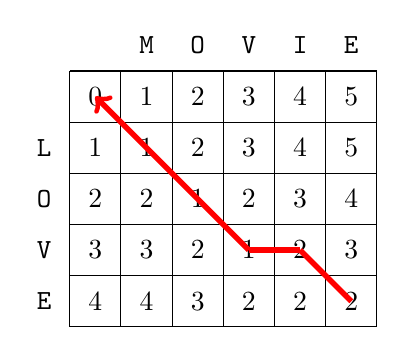
\begin{tikzpicture}[scale=.65]
  \begin{scope}
    \draw (1, -1) grid (7, -6);
    
    \node at (0.5,-2.5) {\texttt{L}};
    \node at (0.5,-3.5) {\texttt{O}};
    \node at (0.5,-4.5) {\texttt{V}};
    \node at (0.5,-5.5) {\texttt{E}};

    \node at (2.5,-0.5) {\texttt{M}};
    \node at (3.5,-0.5) {\texttt{O}};
    \node at (4.5,-0.5) {\texttt{V}};
    \node at (5.5,-0.5) {\texttt{I}};
    \node at (6.5,-0.5) {\texttt{E}};

    \node at (1.5,-1.5) {$0$};
    \node at (1.5,-2.5) {$1$};
    \node at (1.5,-3.5) {$2$};
    \node at (1.5,-4.5) {$3$};
    \node at (1.5,-5.5) {$4$};
    \node at (2.5,-1.5) {$1$};
    \node at (2.5,-2.5) {$1$};
    \node at (2.5,-3.5) {$2$};
    \node at (2.5,-4.5) {$3$};
    \node at (2.5,-5.5) {$4$};
    \node at (3.5,-1.5) {$2$};
    \node at (3.5,-2.5) {$2$};
    \node at (3.5,-3.5) {$1$};
    \node at (3.5,-4.5) {$2$};
    \node at (3.5,-5.5) {$3$};
    \node at (4.5,-1.5) {$3$};
    \node at (4.5,-2.5) {$3$};
    \node at (4.5,-3.5) {$2$};
    \node at (4.5,-4.5) {$1$};
    \node at (4.5,-5.5) {$2$};
    \node at (5.5,-1.5) {$4$};
    \node at (5.5,-2.5) {$4$};
    \node at (5.5,-3.5) {$3$};
    \node at (5.5,-4.5) {$2$};
    \node at (5.5,-5.5) {$2$};
    \node at (6.5,-1.5) {$5$};
    \node at (6.5,-2.5) {$5$};
    \node at (6.5,-3.5) {$4$};
    \node at (6.5,-4.5) {$3$};
    \node at (6.5,-5.5) {$2$};

    \path[draw=red,thick,-,line width=2pt] (6.5,-5.5) -- (5.5,-4.5);
    \path[draw=red,thick,-,line width=2pt] (5.5,-4.5) -- (4.5,-4.5);
    \path[draw=red,thick,->,line width=2pt] (4.5,-4.5) -- (1.5,-1.5);
  \end{scope}
\end{tikzpicture}
\end{center}

\begin{comment}
The last characters of \texttt{LOVE} and \texttt{MOVIE}
are equal, so the edit distance between them
equals the edit distance between \texttt{LOV} and \texttt{MOVI}.
We can use one editing operation to remove the
character \texttt{I} from \texttt{MOVI}.
Thus, the edit distance is one larger than
the edit distance between \texttt{LOV} and \texttt{MOV}, etc.
\end{comment}

\texttt{LOVE}と\texttt{MOVIE}の末尾の文字は同じなので、
これらの編集距離は\texttt{LOV}と\texttt{MOVI}の編集距離は同じである。
次に、\texttt{MOVI}から\texttt{I}を取り除くため1回編集を行う。
そして、\texttt{LOV}と\texttt{MOV}の編集距離は、同様に
変更を行うためもう1増える。

\begin{comment}
\section{Counting tilings}

Sometimes the states of a dynamic programming solution
are more complex than fixed combinations of numbers.
As an example,
consider the problem of calculating
the number of distinct ways to
fill an $n \times m$ grid using
$1 \times 2$ and $2 \times 1$ size tiles.
For example, one valid solution
for the $4 \times 7$ grid is
\end{comment}

\section{敷き詰め方の数え上げ}

動的計画法はしばしば単純な数の組み合わせより
難しい解法になる場合もある。
例として、$n \times m$のグリッドを、
$1 \times 2$または$2 \times 1$の大きさのタイルで敷き詰める
場合の敷き詰め方の数え上げ問題を考える。
例えば、$4 \times 7$のグリッドにおける
1つの敷き詰め方はこの通りである:
\begin{center}
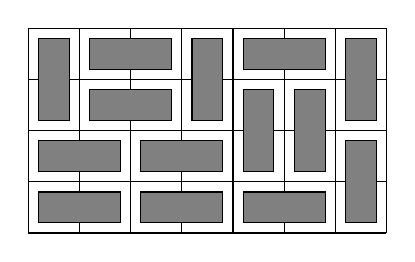
\begin{tikzpicture}[scale=.65]
    \draw (0,0) grid (7,4);
    \draw[fill=gray] (0+0.2,0+0.2) rectangle (2-0.2,1-0.2);
    \draw[fill=gray] (2+0.2,0+0.2) rectangle (4-0.2,1-0.2);
    \draw[fill=gray] (4+0.2,0+0.2) rectangle (6-0.2,1-0.2);
    \draw[fill=gray] (0+0.2,1+0.2) rectangle (2-0.2,2-0.2);
    \draw[fill=gray] (2+0.2,1+0.2) rectangle (4-0.2,2-0.2);
    \draw[fill=gray] (1+0.2,2+0.2) rectangle (3-0.2,3-0.2);
    \draw[fill=gray] (1+0.2,3+0.2) rectangle (3-0.2,4-0.2);
    \draw[fill=gray] (4+0.2,3+0.2) rectangle (6-0.2,4-0.2);

    \draw[fill=gray] (0+0.2,2+0.2) rectangle (1-0.2,4-0.2);
    \draw[fill=gray] (3+0.2,2+0.2) rectangle (4-0.2,4-0.2);
    \draw[fill=gray] (6+0.2,2+0.2) rectangle (7-0.2,4-0.2);
    \draw[fill=gray] (4+0.2,1+0.2) rectangle (5-0.2,3-0.2);
    \draw[fill=gray] (5+0.2,1+0.2) rectangle (6-0.2,3-0.2);
    \draw[fill=gray] (6+0.2,0+0.2) rectangle (7-0.2,2-0.2);

\end{tikzpicture}
\end{center}

\begin{comment}
and the total number of solutions is 781.

The problem can be solved using dynamic programming
by going through the grid row by row.
Each row in a solution can be represented as a
string that contains $m$ characters from the set
$\{\sqcap, \sqcup, \sqsubset, \sqsupset \}$.
For example, the above solution consists of four rows
that correspond to the following strings:
\end{comment}

そしてこの問題の総数は781である。

この問題は、行ごとに処理を進めていく動的計画法で解くことができる。
各行を構成するマスに乗るタイルの形状を、
$\{\sqcap, \sqcup, \sqsubset, \sqsupset \}$からなる
$m$文字の文字列として表すことにしよう。
例えば先ほどの例は、以下の文字列で表現できる:
\begin{itemize}
\item
$\sqcap \sqsubset \sqsupset \sqcap \sqsubset \sqsupset \sqcap$
\item
$\sqcup \sqsubset \sqsupset \sqcup \sqcap \sqcap \sqcup$
\item
$\sqsubset \sqsupset \sqsubset \sqsupset \sqcup \sqcup \sqcap$ 
\item
$\sqsubset \sqsupset \sqsubset \sqsupset \sqsubset \sqsupset \sqcup$
\end{itemize}

\begin{comment}
Let $\texttt{count}(k,x)$ denote the number of ways to
construct a solution for rows $1 \ldots k$
of the grid such that string $x$ corresponds to row $k$.
It is possible to use dynamic programming here,
because the state of a row is constrained
only by the state of the previous row.

A solution is valid if row $1$ does not contain
the character $\sqcup$,
row $n$ does not contain the character $\sqcap$,
and all consecutive rows are \emph{compatible}.
For example, the rows
$\sqcup \sqsubset \sqsupset \sqcup \sqcap \sqcap \sqcup$ and
$\sqsubset \sqsupset \sqsubset \sqsupset \sqcup \sqcup \sqcap$ 
are compatible, while the rows
$\sqcap \sqsubset \sqsupset \sqcap \sqsubset \sqsupset \sqcap$ and
$\sqsubset \sqsupset \sqsubset \sqsupset \sqsubset \sqsupset \sqcup$
are not compatible.
\end{comment}

$\texttt{count}(k,x)$を、グリッドのうち$1 \ldots k$行の範囲は
すでにタイルが埋められており、かつ$k$行目の状態が
文字列$x$に相当する埋め方をされている場合の組み合わせとする。
ここで、行の状態は手前の行の状態をもとに構築できるので、
動的計画法を活用することができる。

有効な解は、まず$1$行目が文字$\sqcup$,を含まず、
$n$行目が文字$\sqcap$を含まず、
連続する行が互いに\emph{矛盾しない}.ことである。
例えば2つの行
$\sqcup \sqsubset \sqsupset \sqcup \sqcap \sqcap \sqcup$と
$\sqsubset \sqsupset \sqsubset \sqsupset \sqcup \sqcup \sqcap$ 
は矛盾しないが、
$\sqcap \sqsubset \sqsupset \sqcap \sqsubset \sqsupset \sqcap$と
$\sqsubset \sqsupset \sqsubset \sqsupset \sqsubset \sqsupset \sqcup$
の行は矛盾する。

\begin{comment}
Since a row consists of $m$ characters and there are
four choices for each character, the number of distinct
rows is at most $4^m$.
Thus, the time complexity of the solution is
$O(n 4^{2m})$ because we can go through the
$O(4^m)$ possible states for each row,
and for each state, there are $O(4^m)$
possible states for the previous row.
In practice, it is a good idea to rotate the grid
so that the shorter side has length $m$,
because the factor $4^{2m}$ dominates the time complexity.

It is possible to make the solution more efficient
by using a more compact representation for the rows.
It turns out that it is sufficient to know which
columns of the previous row contain the upper square
of a vertical tile.
Thus, we can represent a row using only characters
$\sqcap$ and $\Box$, where $\Box$ is a combination
of characters
$\sqcup$, $\sqsubset$ and $\sqsupset$.
Using this representation, there are only
$2^m$ distinct rows and the time complexity is
$O(n 2^{2m})$.
\end{comment}

1つの行の表現に$m$個の文字が必要で、
各文字4通りの組み合わせがあるので、
行の状態は最大$4^m$通り考えられる。
そのため、この解法の時間計算量は$O(n 4^{2m})$である。
というのも、処理対象の行と手前の行はそれぞれ$O(4^m)$通りの
状態を持つためである。
この計算量は$4^{2m}$の箇所が支配的なので、
実際、グリッドを回転させ、$n$より$m$が小さくなるように
するのは良いアイデアである。

行に対し、よりコンパクトな表現を用いることで、
より効率化することもできる。
前の行の情報として必要なのは、各マスが$\sqcap$かどうかだけである。
よって、行の状態を$\sqcap$と$\Box$の2種類の文字だけ
考えるようにできる。(ここで$\Box$は$\sqcup$, $\sqsubset$, $\sqsupset$の
いずれかに相当する)
この表現により、行の状態が$2^m$通りで表現できるため、
全体の時間計算量は$O(n 2^{2m})$となる。

\begin{comment}
As a final note, there is also a surprising direct formula
for calculating the number of tilings\footnote{Surprisingly,
this formula was discovered in 1961 by two research teams \cite{kas61,tem61}
that worked independently.}:
\[ \prod_{a=1}^{\lceil n/2 \rceil} \prod_{b=1}^{\lceil m/2 \rceil} 4 \cdot (\cos^2 \frac{\pi a}{n + 1} + \cos^2 \frac{\pi b}{m+1})\]
This formula is very efficient, because it calculates
the number of tilings in $O(nm)$ time,
but since the answer is a product of real numbers,
a problem when using the formula is
how to store the intermediate results accurately.
\end{comment}

最後に付録として、この敷き詰め問題の驚くべき式を紹介する
\footnote{驚くべきことに、この式は偶然2人の研究チームが同じ年に発見した\cite{kas61,tem61}}:
\[ \prod_{a=1}^{\lceil n/2 \rceil} \prod_{b=1}^{\lceil m/2 \rceil} 4 \cdot (\cos^2 \frac{\pi a}{n + 1} + \cos^2 \frac{\pi b}{m+1})\]

この式は、$O(nm)$で計算できるので非常に高速である。
しかし計算過程で小数値の乗算を含むため、
計算過程でどうやって中間状態を正確に保持するかという問題は残る。
